\documentclass[12pt, a4paper, lithuanian]{article}
\usepackage[utf8]{inputenc}
\def\LTfontencoding{L7x}
\usepackage[\LTfontencoding]{fontenc}
\usepackage[lithuanian]{babel}
\usepackage{PhDReport}
\usepackage{cite}
\usepackage{amsmath}
\usepackage{bm}
\usepackage{amsfonts}
\usepackage{float}
\usepackage{graphicx}
\usepackage{color}
\usepackage{listings}
\usepackage{wrapfig}
\usepackage{algpseudocode}
\usepackage{algorithm}
\usepackage{algorithmicx}
\usepackage{caption}
\usepackage{subfig}
\usepackage{datetime}

\universitytitle{Vilniaus universitetas}
\departmenttitle{Matematikos ir informatikos institutas}
\departmentdetails{VU Matematikos ir informatikos institutas, Akademijos g. 4,
Vilnius LT-08663 \\ www.mii.lt}
\universitylogo{img/vu_logo}
\departmentlogo{img/mii_logo}
\date{\the\year\ m.\monthlt[\month]}
\scientifictrend{Informatikos inžinerija (07 T)}
\reportid{MII-DS-07T-\shortyear-<ataskaitos nr.>}

\title{<temos pavadinimas>}
\author{<Autorius>}

\begin{document}

\maketitle

\sectionnonumnocontent{Santrauka}\noindent
............

\keywords{....., .....}

\tableofcontents

\section{Įvadas}

\section{<ataskaitos pagrindinė dalis>}
Ataskaitoje dedama medžiaga, kurią doktorantas buvo įsipareigojęs parengti per
ataskaitinį periodą (parašyti disertacijos skyrių, parengti kokią nors metodiką
ar pan.; gali būti parengtų spaudai straipsnių tekstai). Pas ką plane tokių
įsipareigojimų nebuvo, mokslinės ataskaitos rengti nebūtina.

\subsection{<ataskaitos poskyrio pavyzdys>}
Citavimo pavyzdys \cite{VP}.

\section{Literatūra}
Autoriaus publikuoti straipsniai ir knygos.

\bibliography{bibliografija}

\appendix
\section{Algoritmų palyginamųjų eksperimentų rezultatų lentelė}
% tablesgenerator.com - konvertuoja skaičiuoklės, pvz. excel, lentelę į LaTeX
\begin{table}[H]
  \centering
  \caption{Palyginamųjų eksperimentų rezultatai su realaus pasaulio duomenimis.
    Palyginti \emph{Algoritmas A} ir \emph{Algoritmas B} pagal $\bar{x}$ ir $\sigma^{2}$ dydžius.}
  {\begin{tabular}{|l|c|c|} \hline
    Algoritmas    & $\bar{x}$ & $\sigma^{2}$ \\
    \hline
    Algoritmas A  & 1.6335    & 0.5584       \\
    Algoritmas B  & 1.7395    & 0.5647       \\
    \hline
  \end{tabular}}
  \label{tab:table example}
\end{table}

\pagebreak

\section{Sudėtingų geometrinių paviršių sankirtos paveikslėlis}
\begin{figure}[H]
    \centering
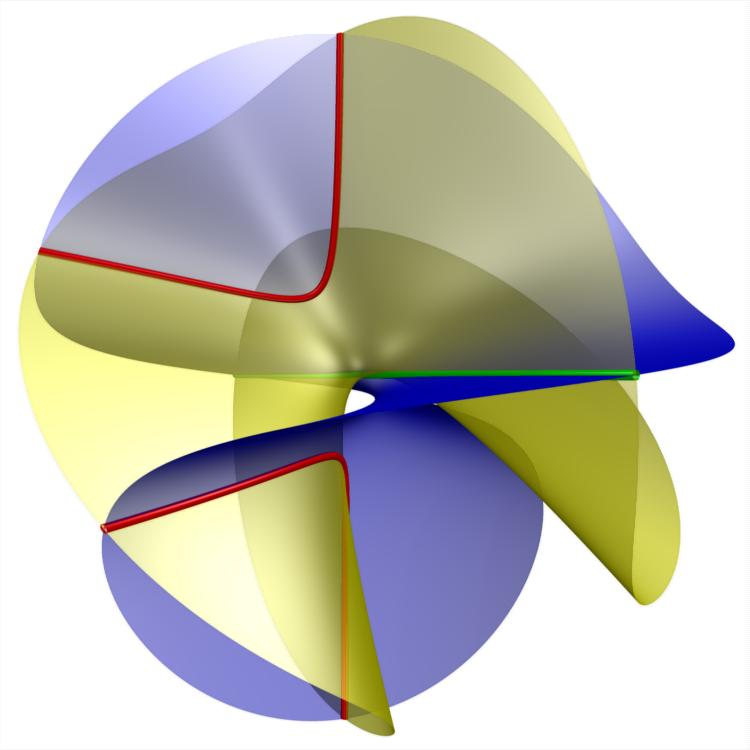
\includegraphics[scale=0.13]{img/cones}
\caption{Paveikslėlio pavyzdys}
\end{figure}

\end{document}
